\chapter{نمودارهای توالی طراحی}


نمودارهای توالی طراحی مربوط به هریک از موارد کاربرد (با نام مشابه) به تفکیک زیرسیستم در این بخش ارائه می‌شود.



\begin{figure}[ht!]
	\centering
	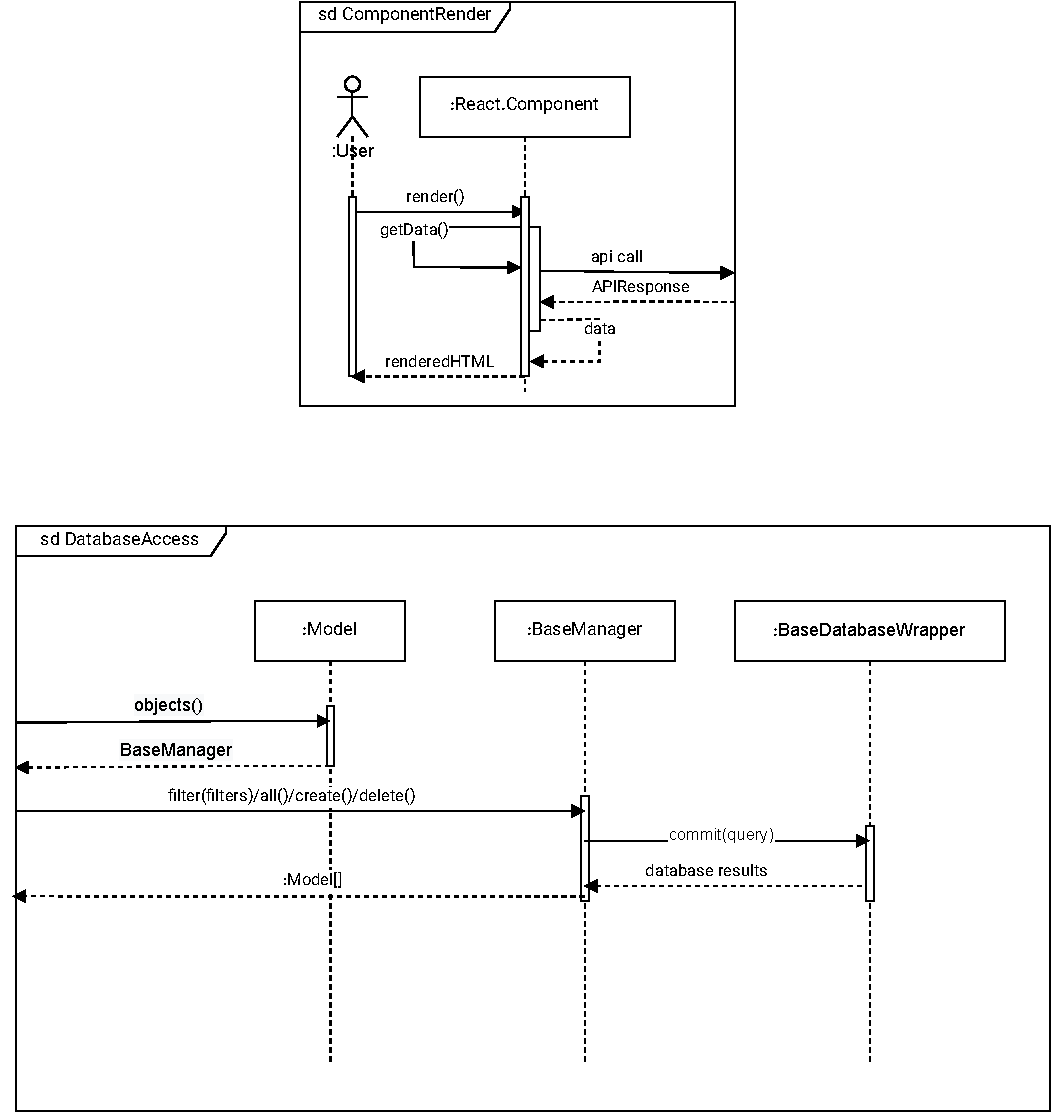
\includegraphics[scale=0.8]{figs/design-sequence/reusable.pdf}
	\caption{قطعه نمودارهای توالی قابل استفاده مجدد}
\end{figure}
\FloatBarrier
\newpage

\newpage
\section{زیرسیستم کاربری}

\eject \pdfpagewidth=12in \pdfpageheight=7in
\begin{figure}[ht!]
	\centering
	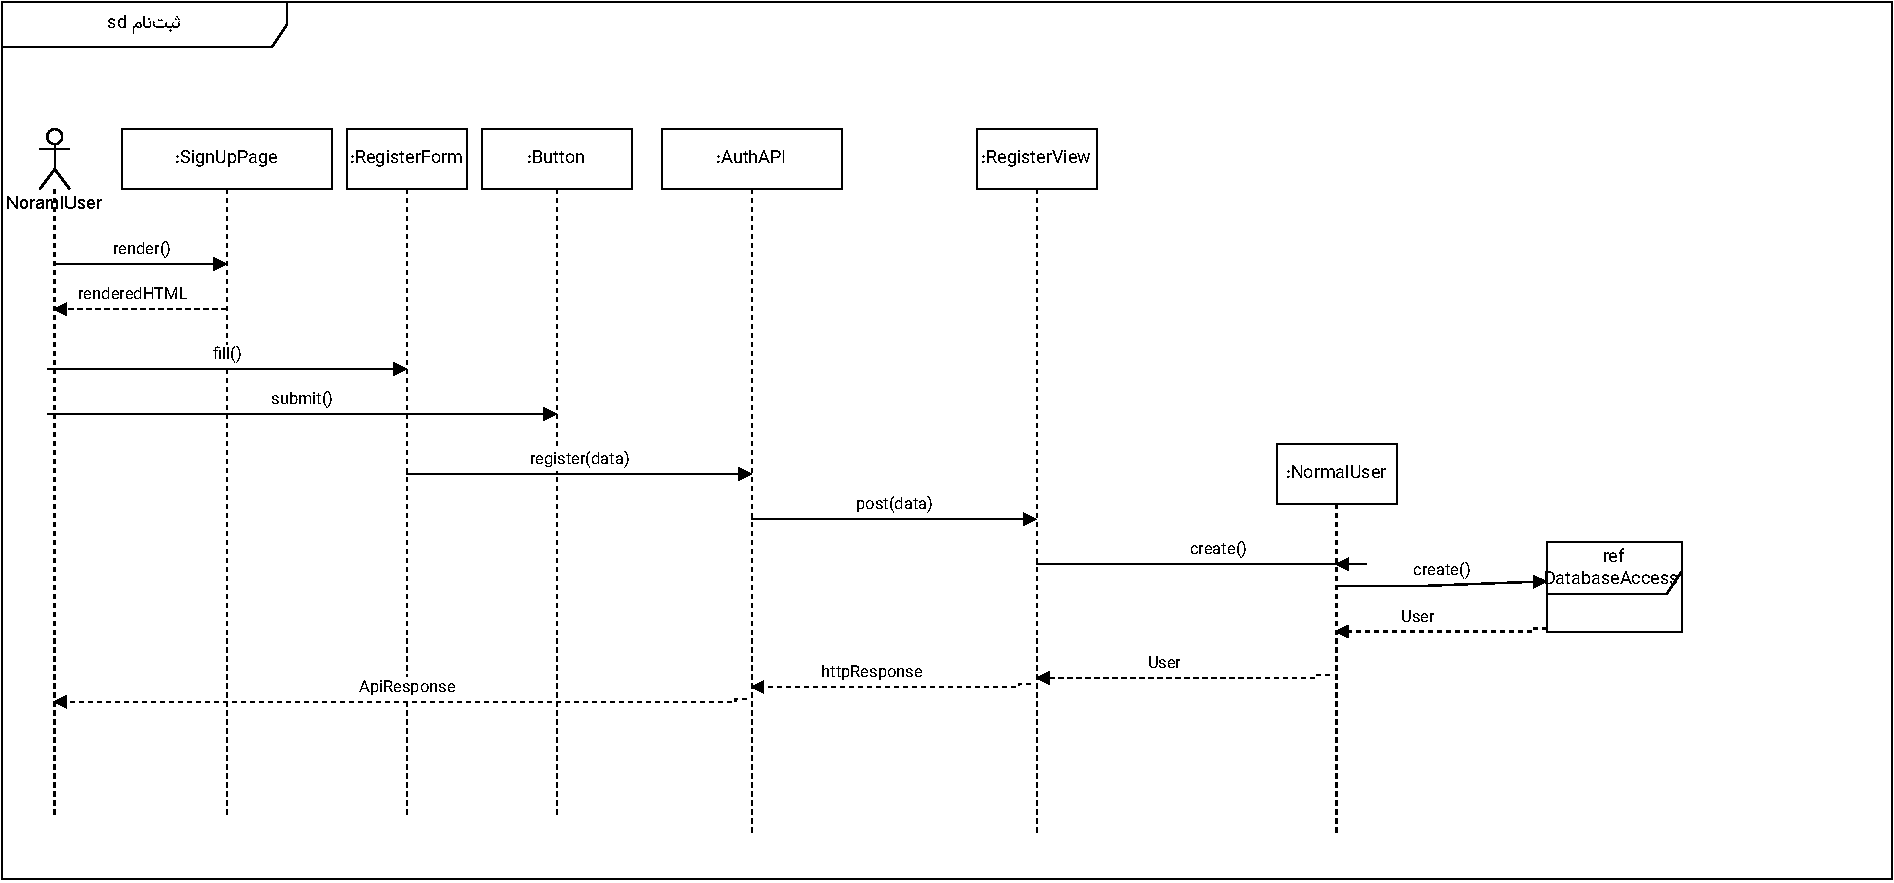
\includegraphics[scale=0.8]{figs/design-sequence/3-1.pdf}
	\caption{نمودار توالی: ثبت نام}
\end{figure}
\FloatBarrier
\newpage

\eject \pdfpagewidth=11in \pdfpageheight=7in
\begin{figure}[ht!]
	\centering
	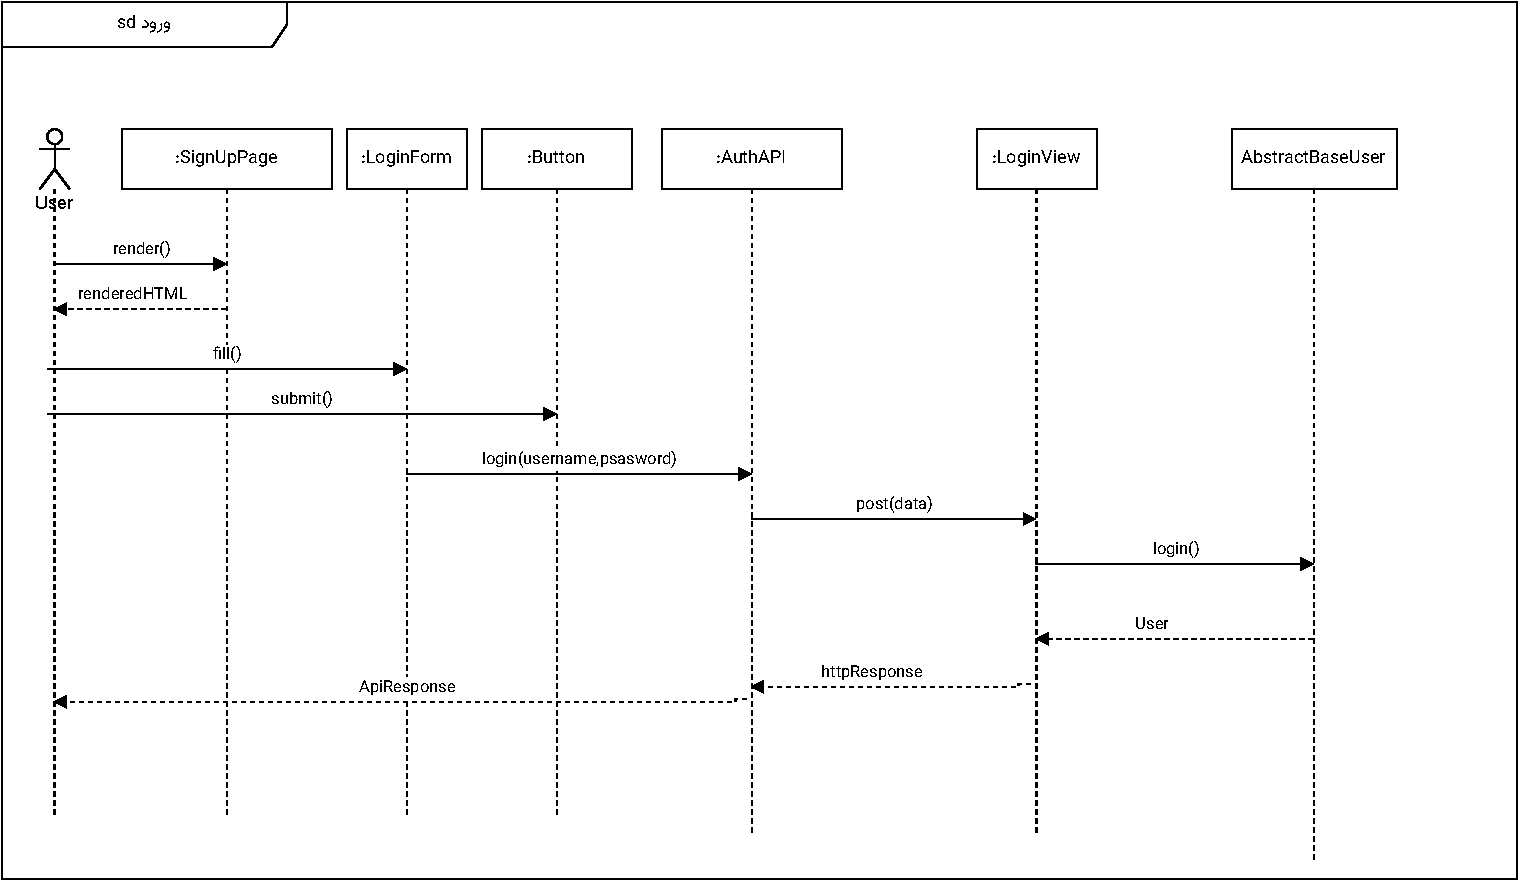
\includegraphics[scale=0.8]{figs/design-sequence/3-2.pdf}
	\caption{نمودار توالی: ورود}
\end{figure}
\FloatBarrier
\newpage

\section{زیرسیستم خدمت‌دهی}

\eject \pdfpagewidth=11in \pdfpageheight=7in

\begin{figure}[ht!]
	\centering
	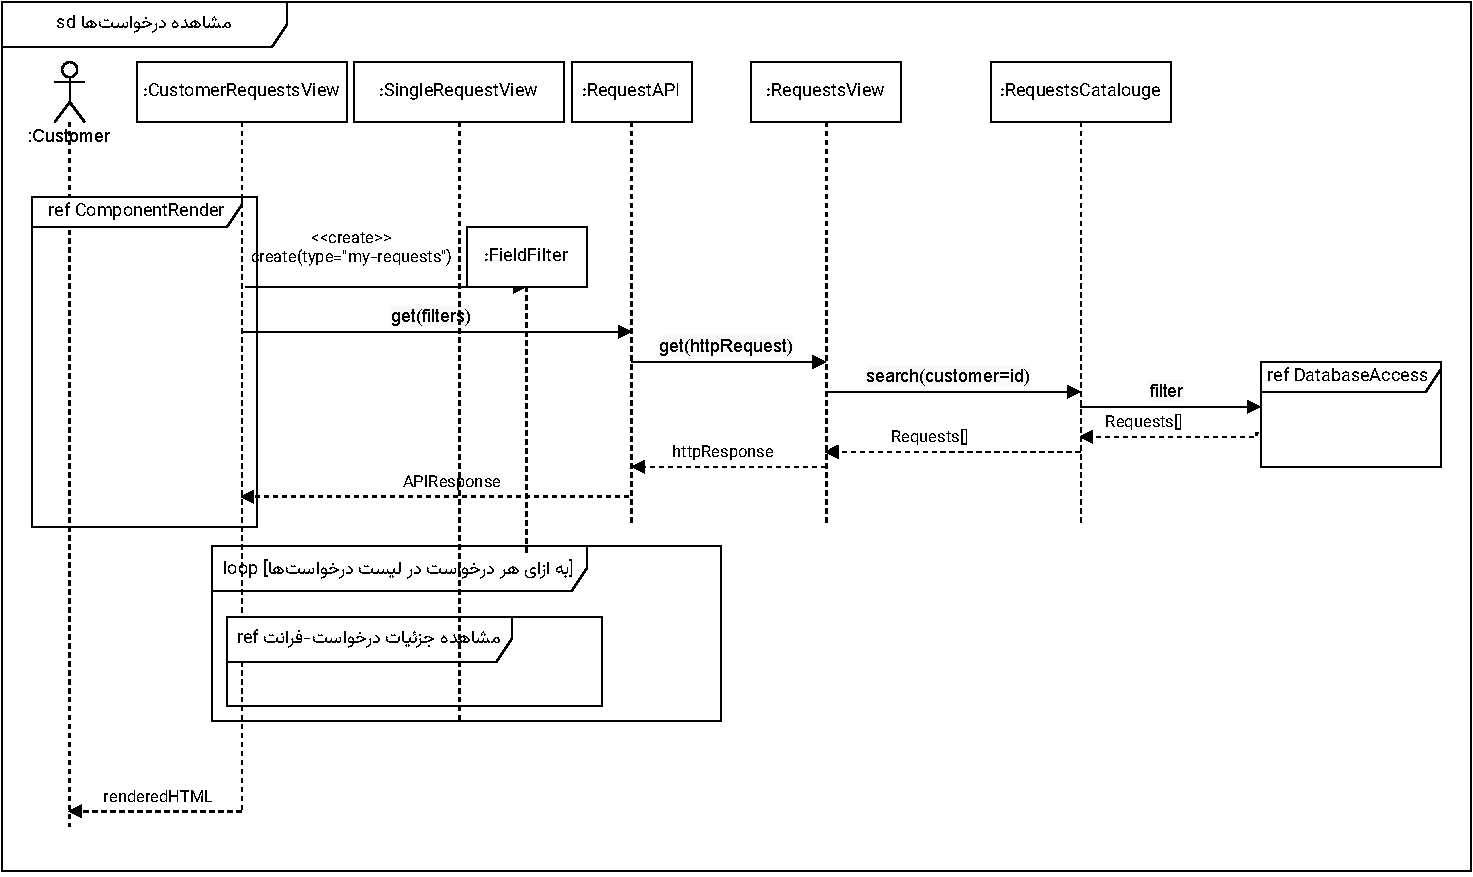
\includegraphics[scale=0.8]{figs/design-sequence/3-10.pdf}
	\caption{نمودار توالی: مشاهده درخواست‌ها}
\end{figure}
\FloatBarrier
\newpage

\eject \pdfpagewidth=10in \pdfpageheight=10in

\begin{figure}[ht!]
	\centering
	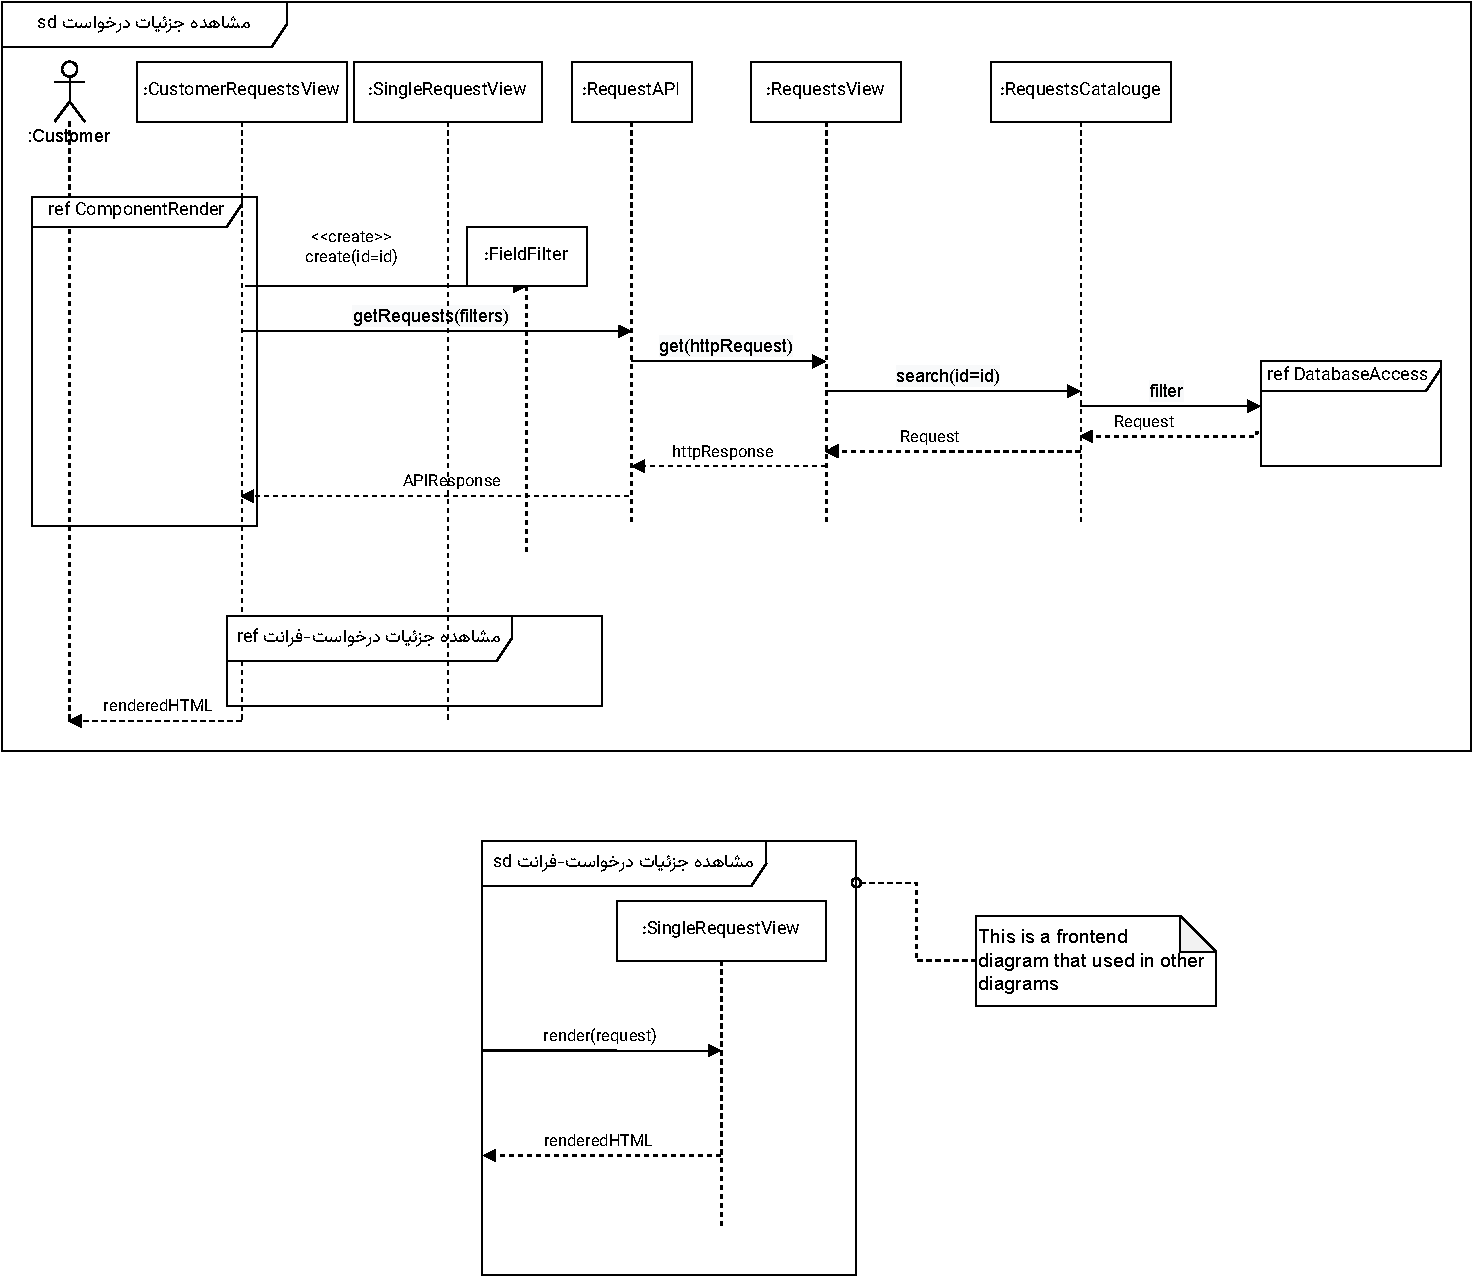
\includegraphics[scale=0.8]{figs/design-sequence/3-11.pdf}
	\caption{نمودار توالی: مشاهده جزئیات درخواست}
\end{figure}
\FloatBarrier
\newpage

\eject \pdfpagewidth=15in \pdfpageheight=12in

\begin{figure}[ht!]
	\centering
	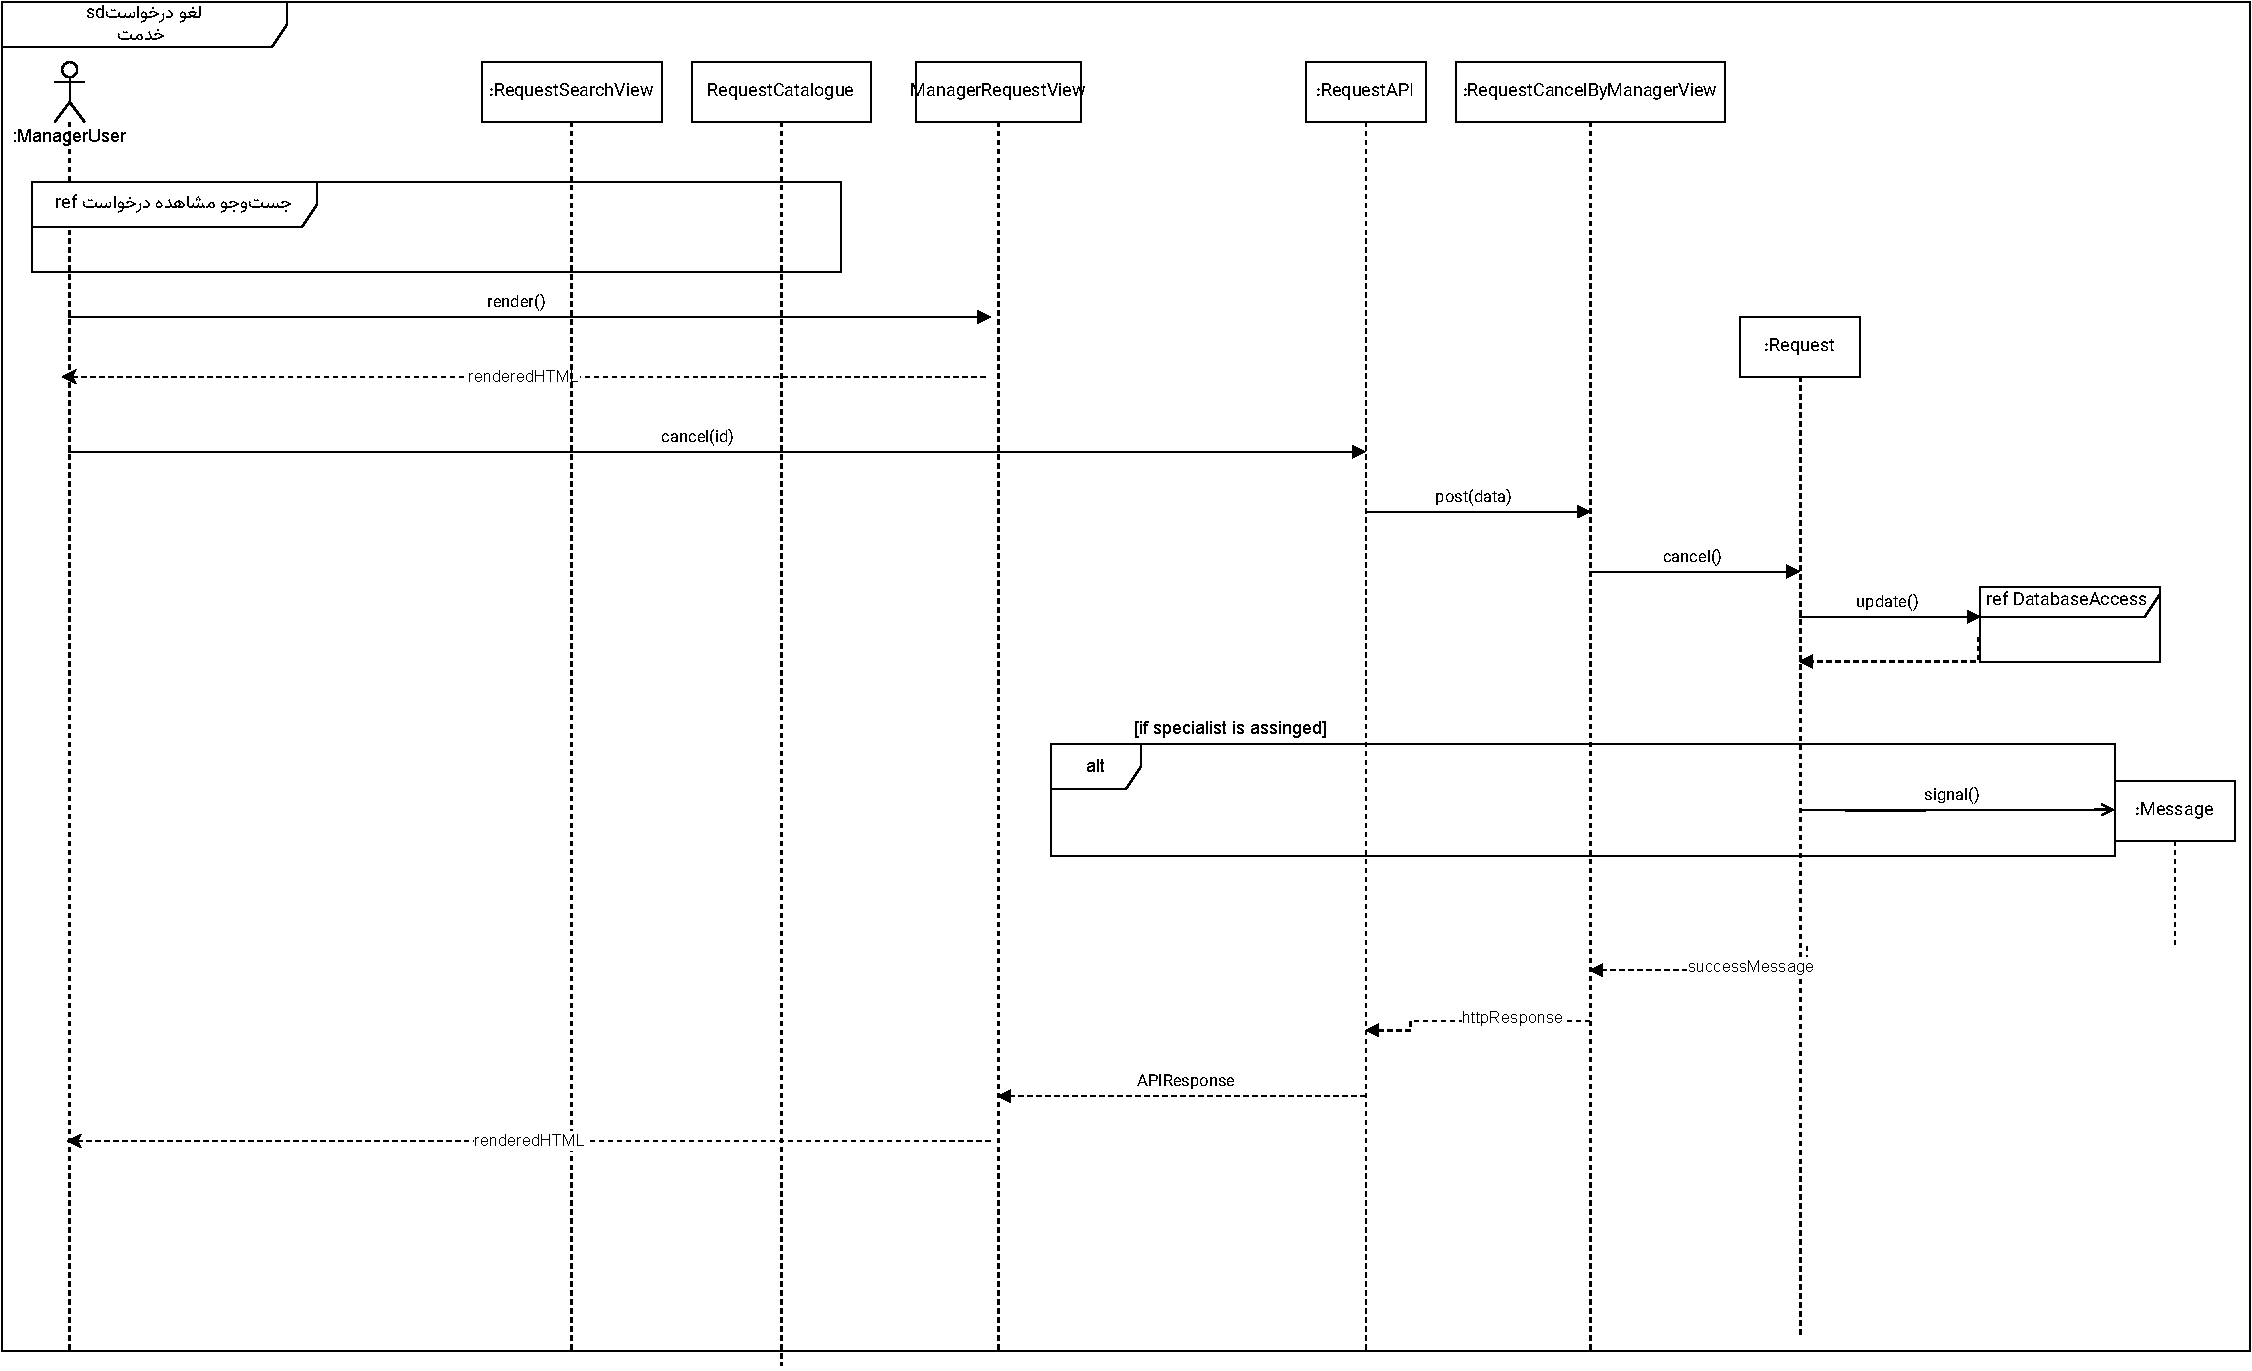
\includegraphics[scale=0.8]{figs/design-sequence/3-16.pdf}
	\caption{نمودار توالی: لغو درخواست خدمت}
\end{figure}
\FloatBarrier
\newpage


\eject \pdfpagewidth=12in \pdfpageheight=8in

\begin{figure}[ht!]
	\centering
	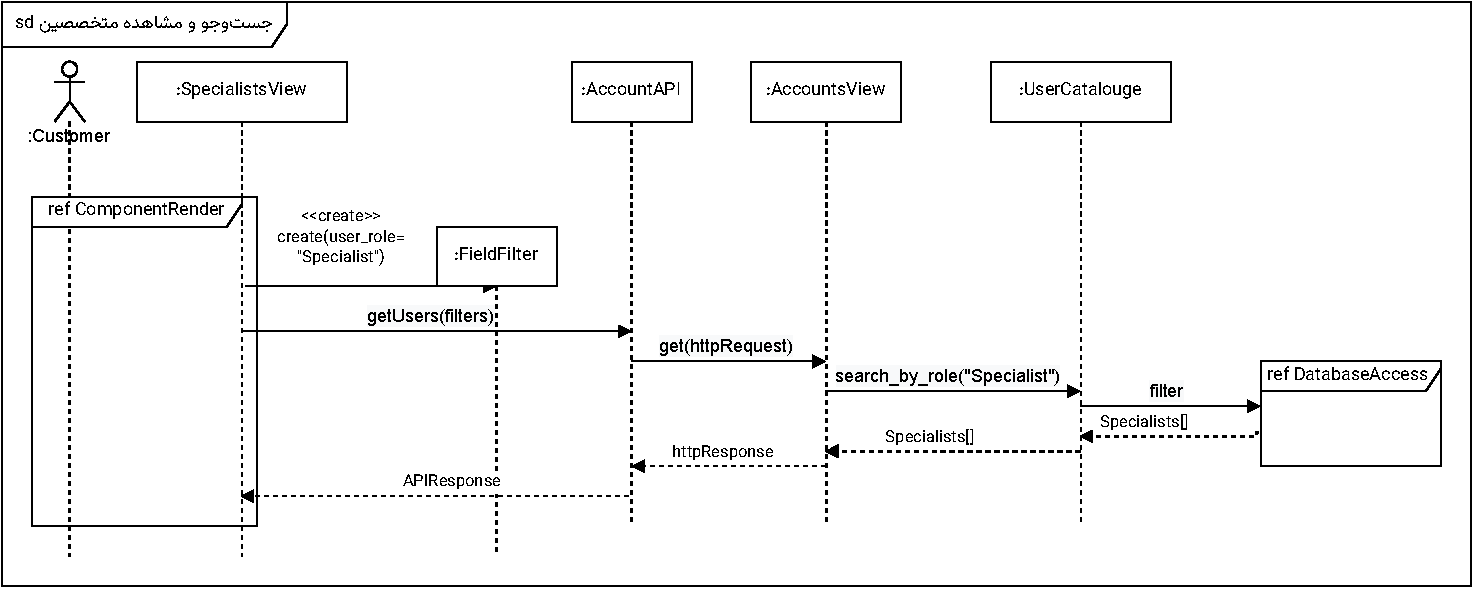
\includegraphics[scale=0.8]{figs/design-sequence/3-17.pdf}
	\caption{نمودار توالی: جست‌وجو و مشاهده متخصصین}
\end{figure}
\FloatBarrier
\newpage

\eject \pdfpagewidth=15in \pdfpageheight=12in

\begin{figure}[ht!]
	\centering
	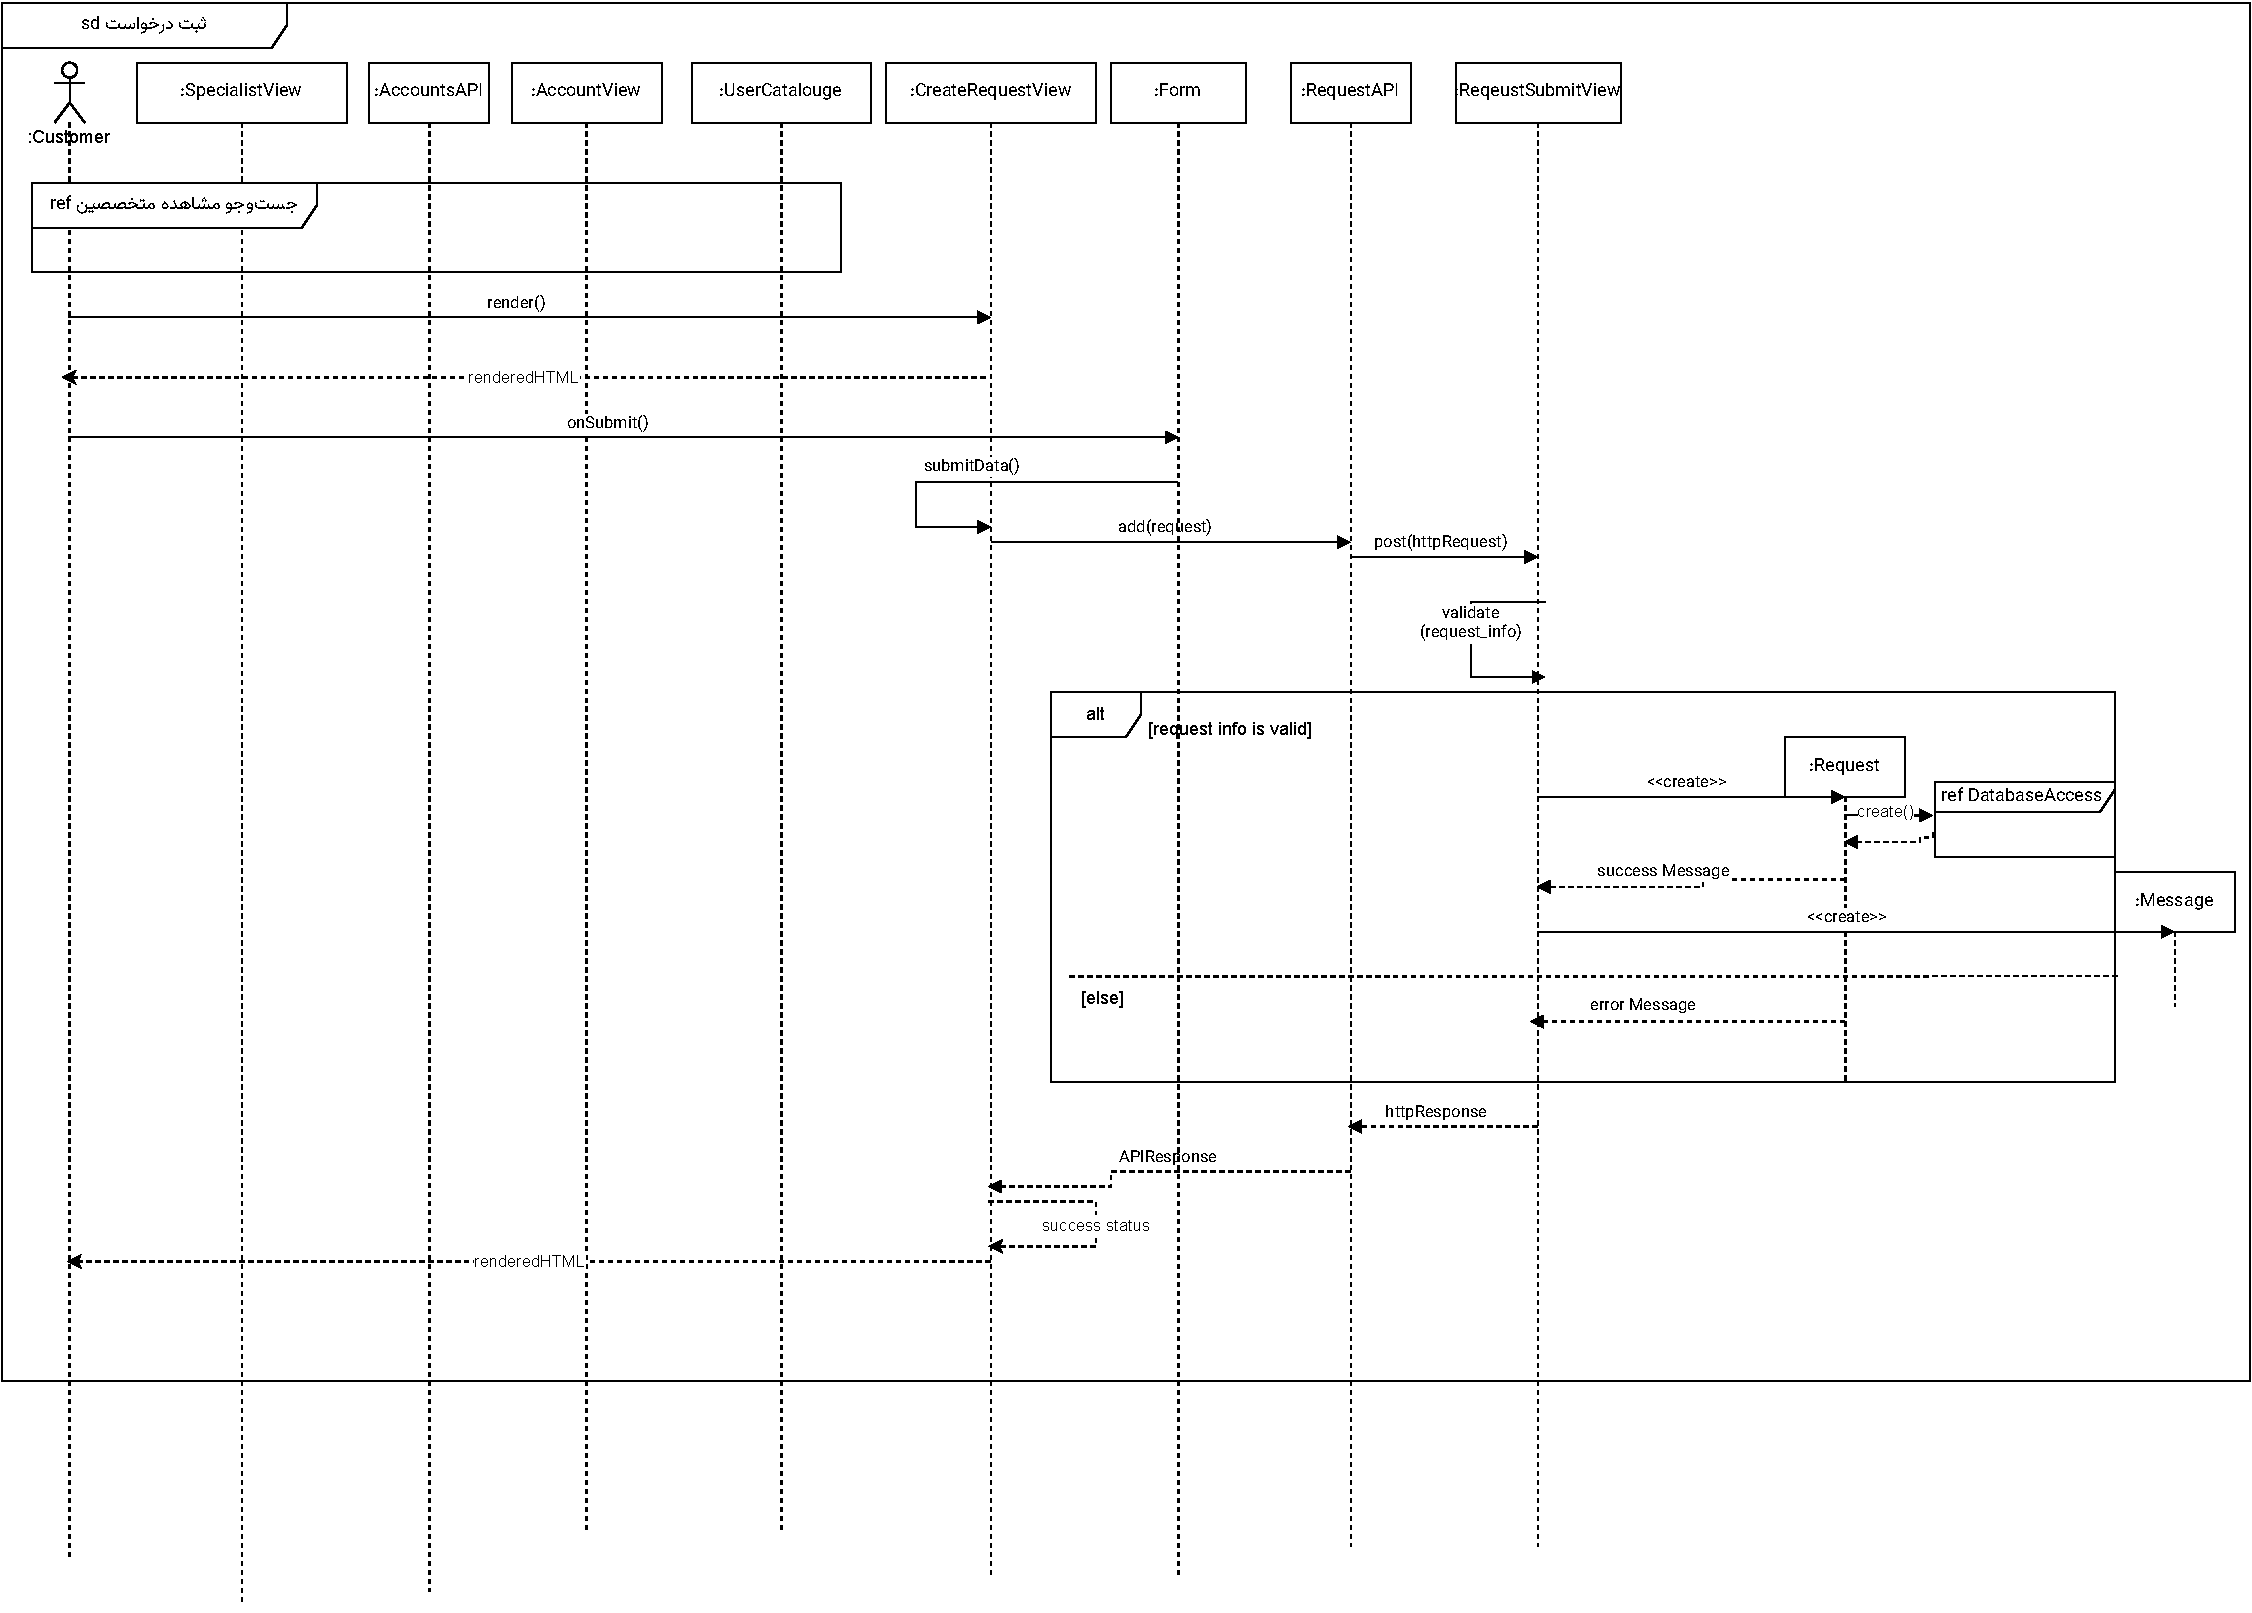
\includegraphics[scale=0.8]{figs/design-sequence/3-18.pdf}
	\caption{نمودار توالی: ثبت درخواست}
\end{figure}
\FloatBarrier
\newpage



\section{زیرسیستم بازخورد}

\eject \pdfpagewidth=17in \pdfpageheight=8in

\begin{figure}[ht!]
	\centering
	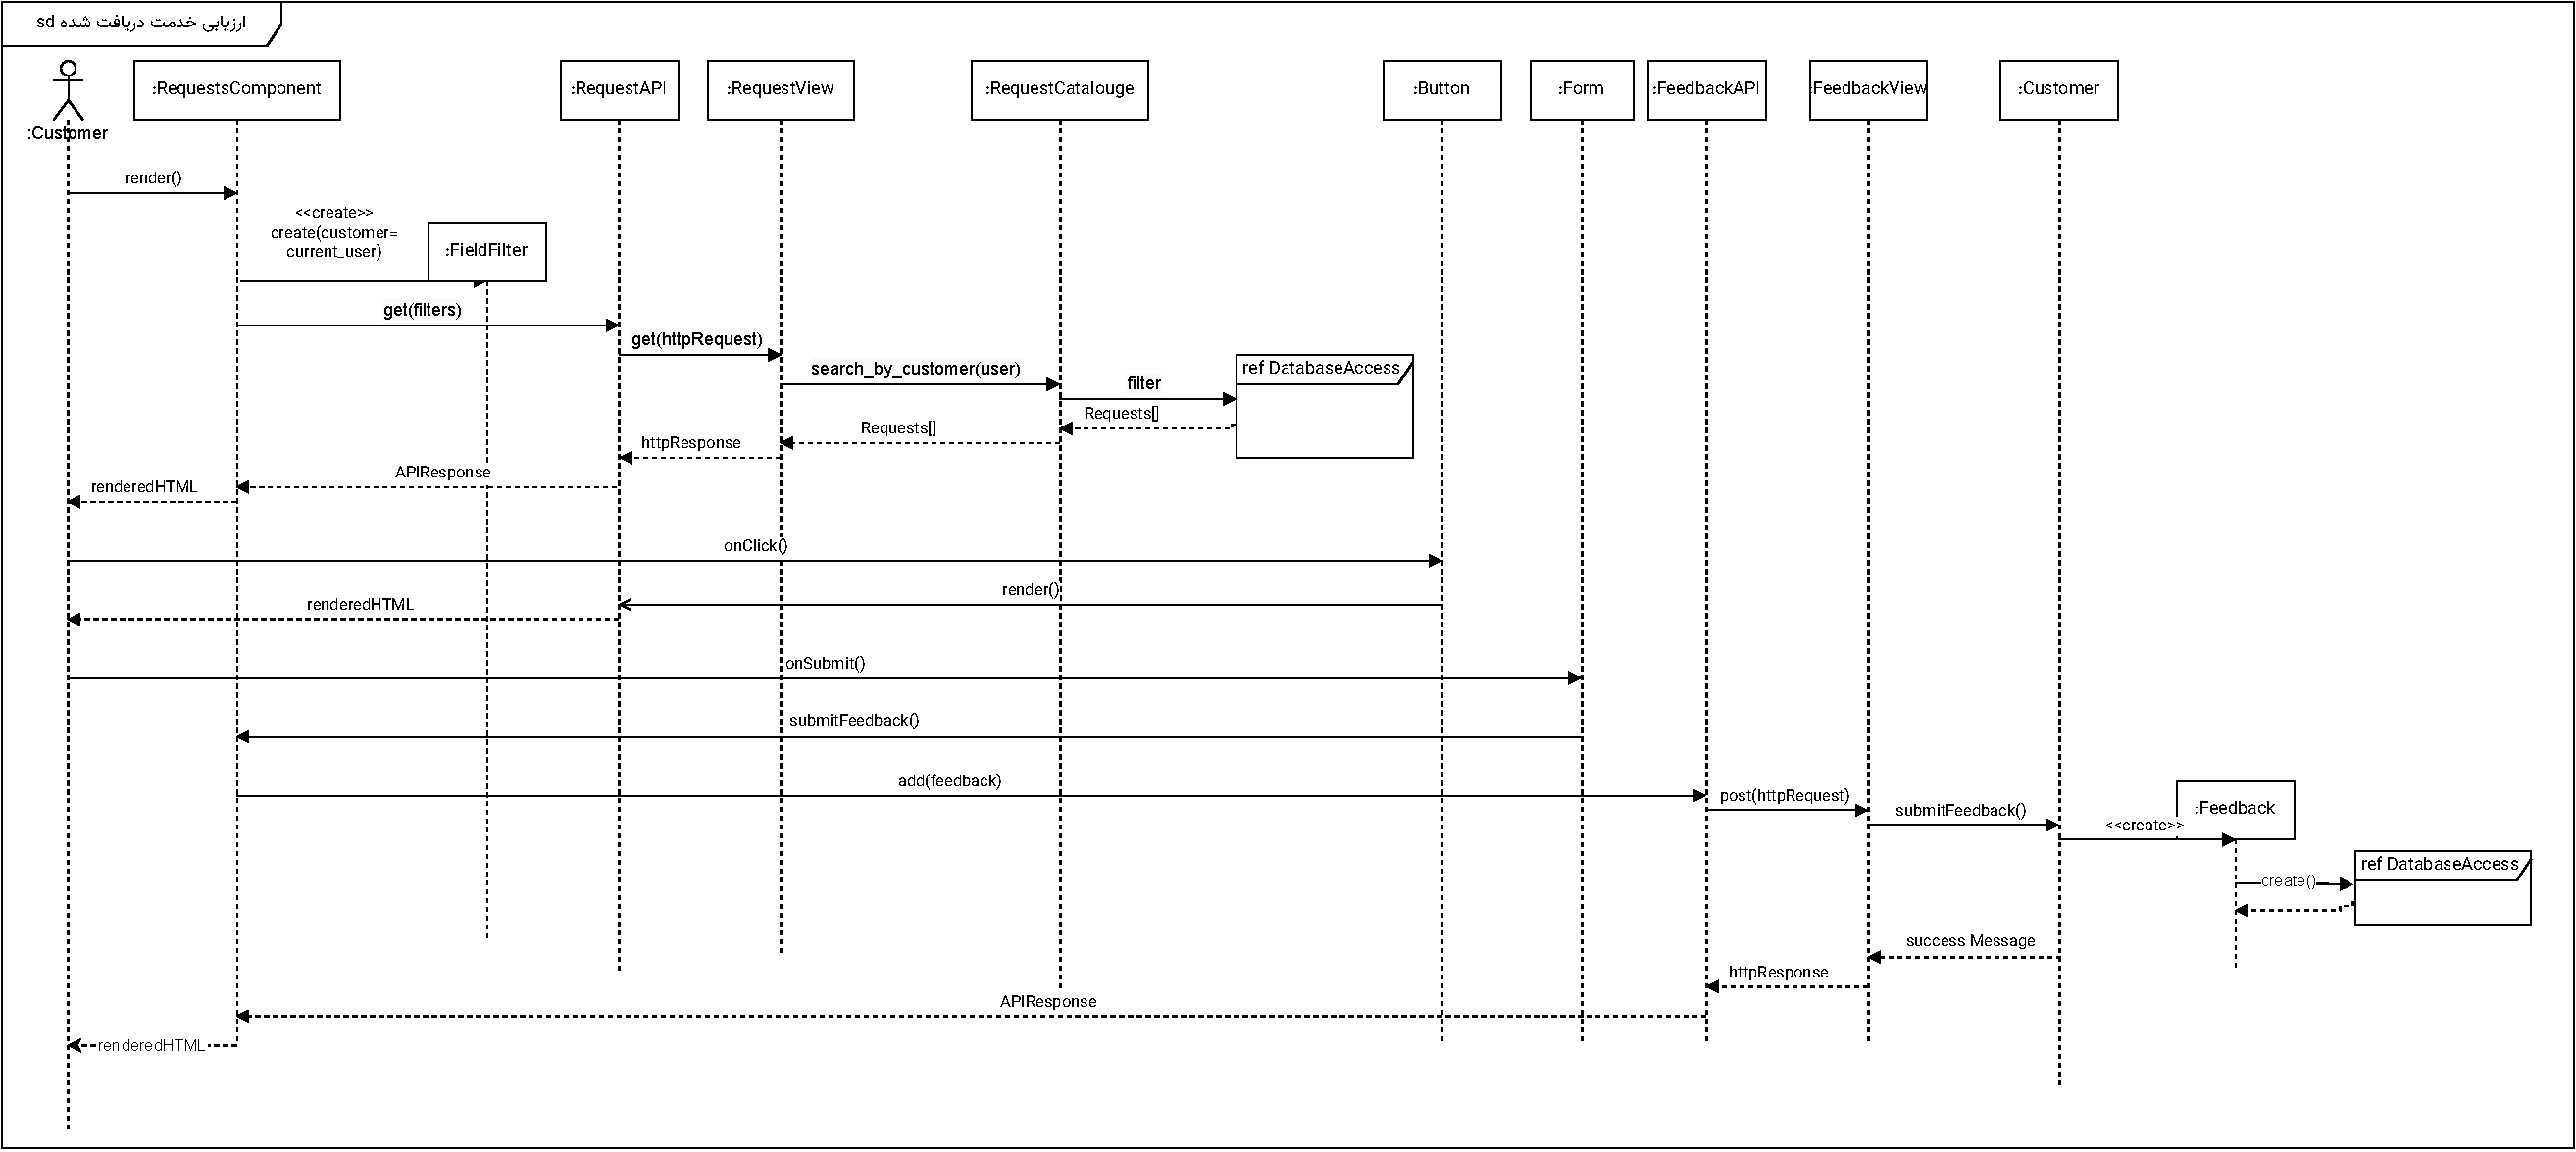
\includegraphics[scale=0.8]{figs/design-sequence/3-24.pdf}
	\caption{نمودار توالی: ارزیابی خدمت دریافت شده}
\end{figure}
\FloatBarrier
\newpage

\eject \pdfpagewidth=17in \pdfpageheight=8in


\begin{figure}[ht!]
	\centering
	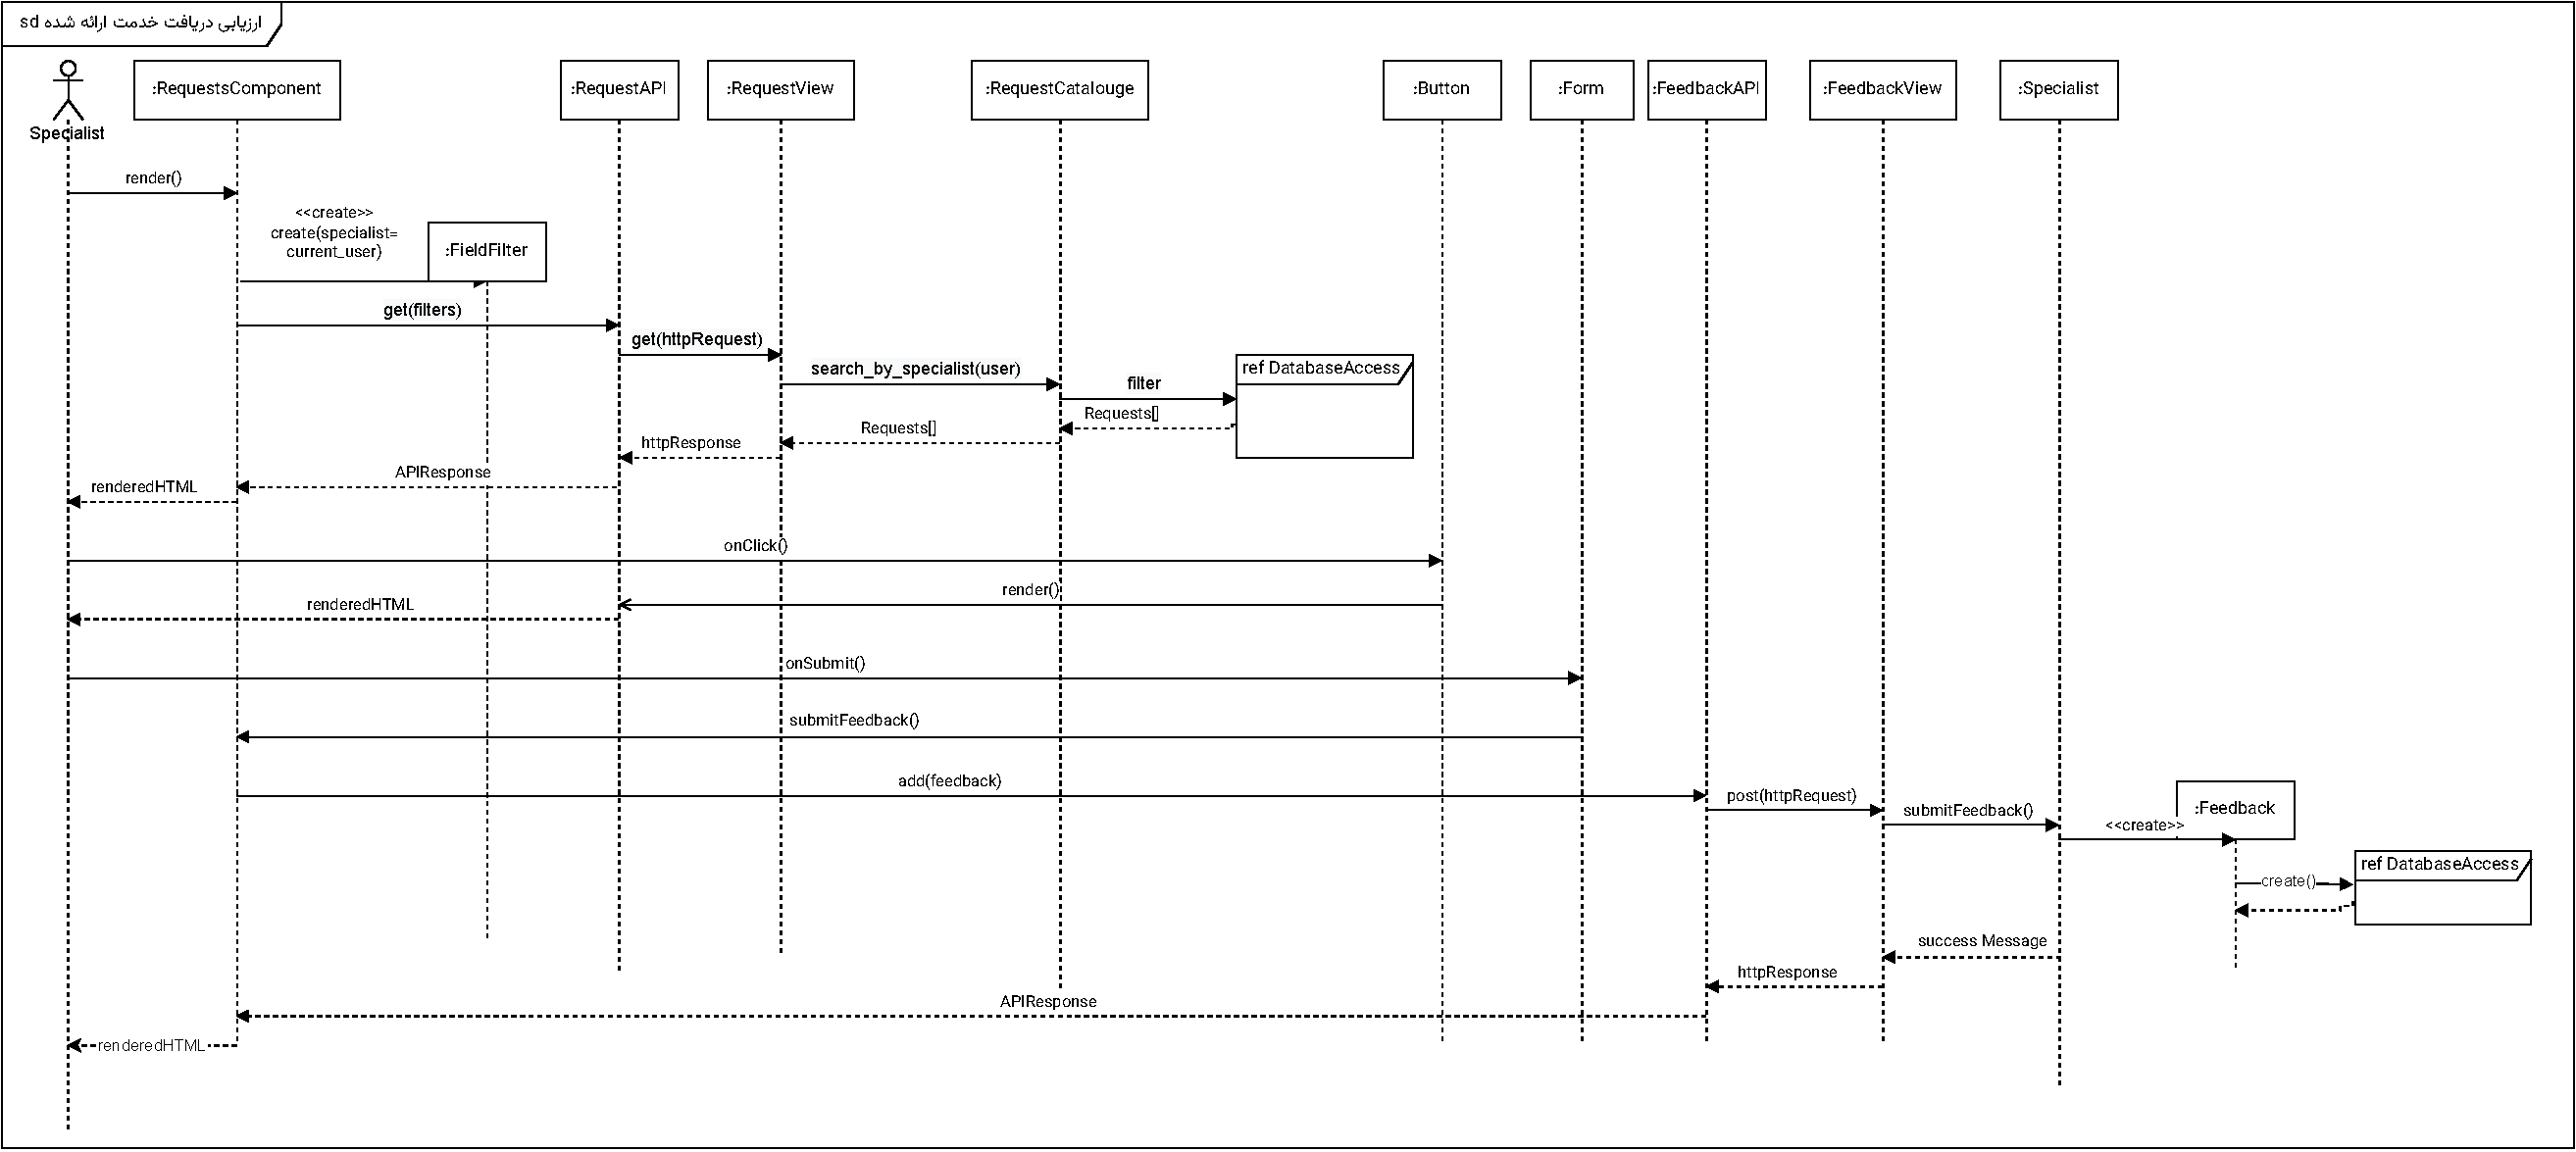
\includegraphics[scale=0.8]{figs/design-sequence/3-25.pdf}
	\caption{نمودار توالی: ارزیابی دریافت خدمت ارائه شده}
\end{figure}
\FloatBarrier
\newpage

\eject \pdfpagewidth=13in \pdfpageheight=6in


\begin{figure}[ht!]
	\centering
	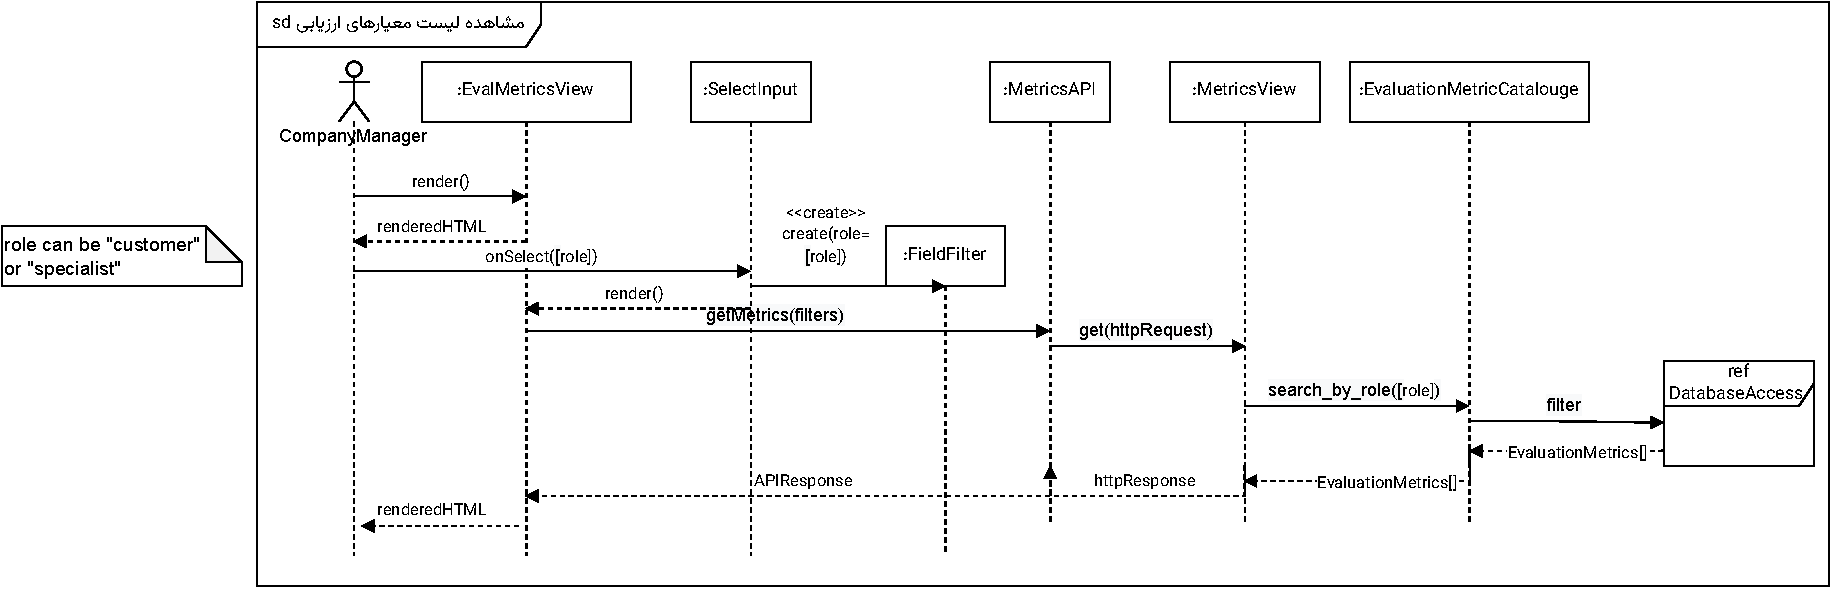
\includegraphics[scale=0.8]{figs/design-sequence/3-26.pdf}
	\caption{نمودار توالی: مشاهده لیست معیارهای ارزیابی}
\end{figure}
\FloatBarrier
\newpage

\eject \pdfpagewidth=10in \pdfpageheight=8in

\begin{figure}[ht!]
	\centering
	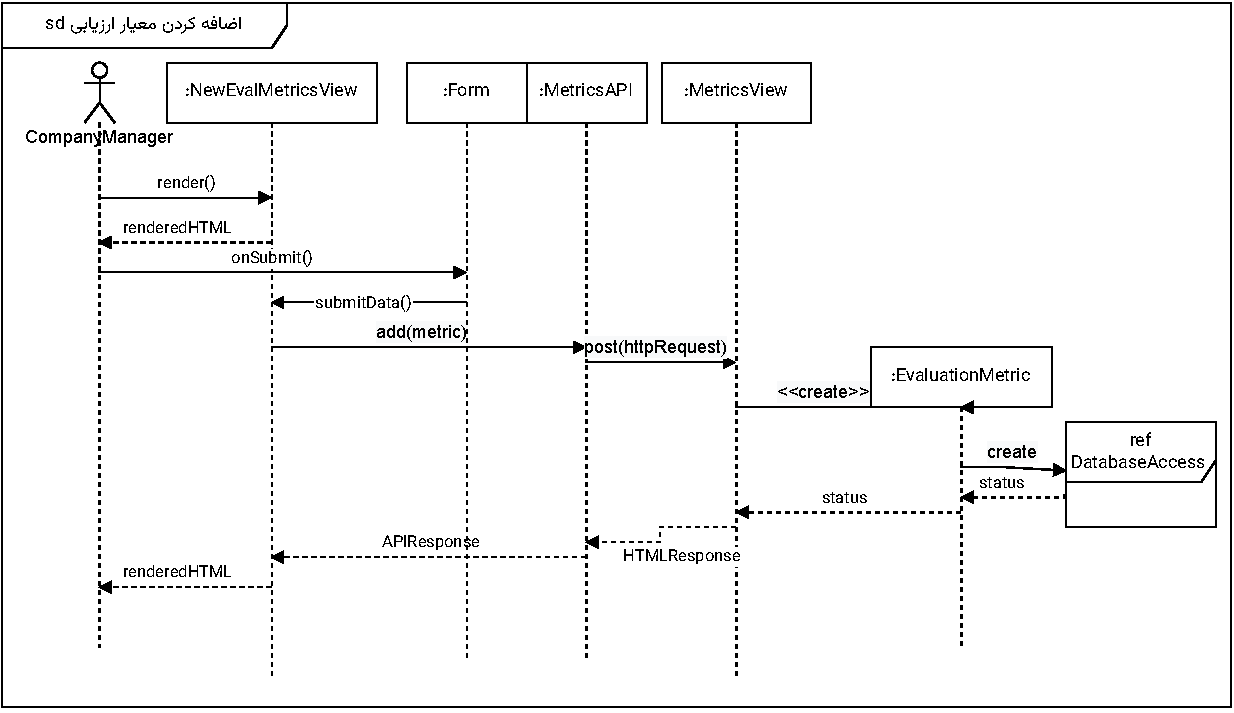
\includegraphics[scale=0.8]{figs/design-sequence/3-27.pdf}
	\caption{نمودار توالی: اضافه کردن معیار ارزیابی}
\end{figure}
\FloatBarrier
\newpage

\eject \pdfpagewidth=12in \pdfpageheight=11in

\begin{figure}[ht!]
	\centering
	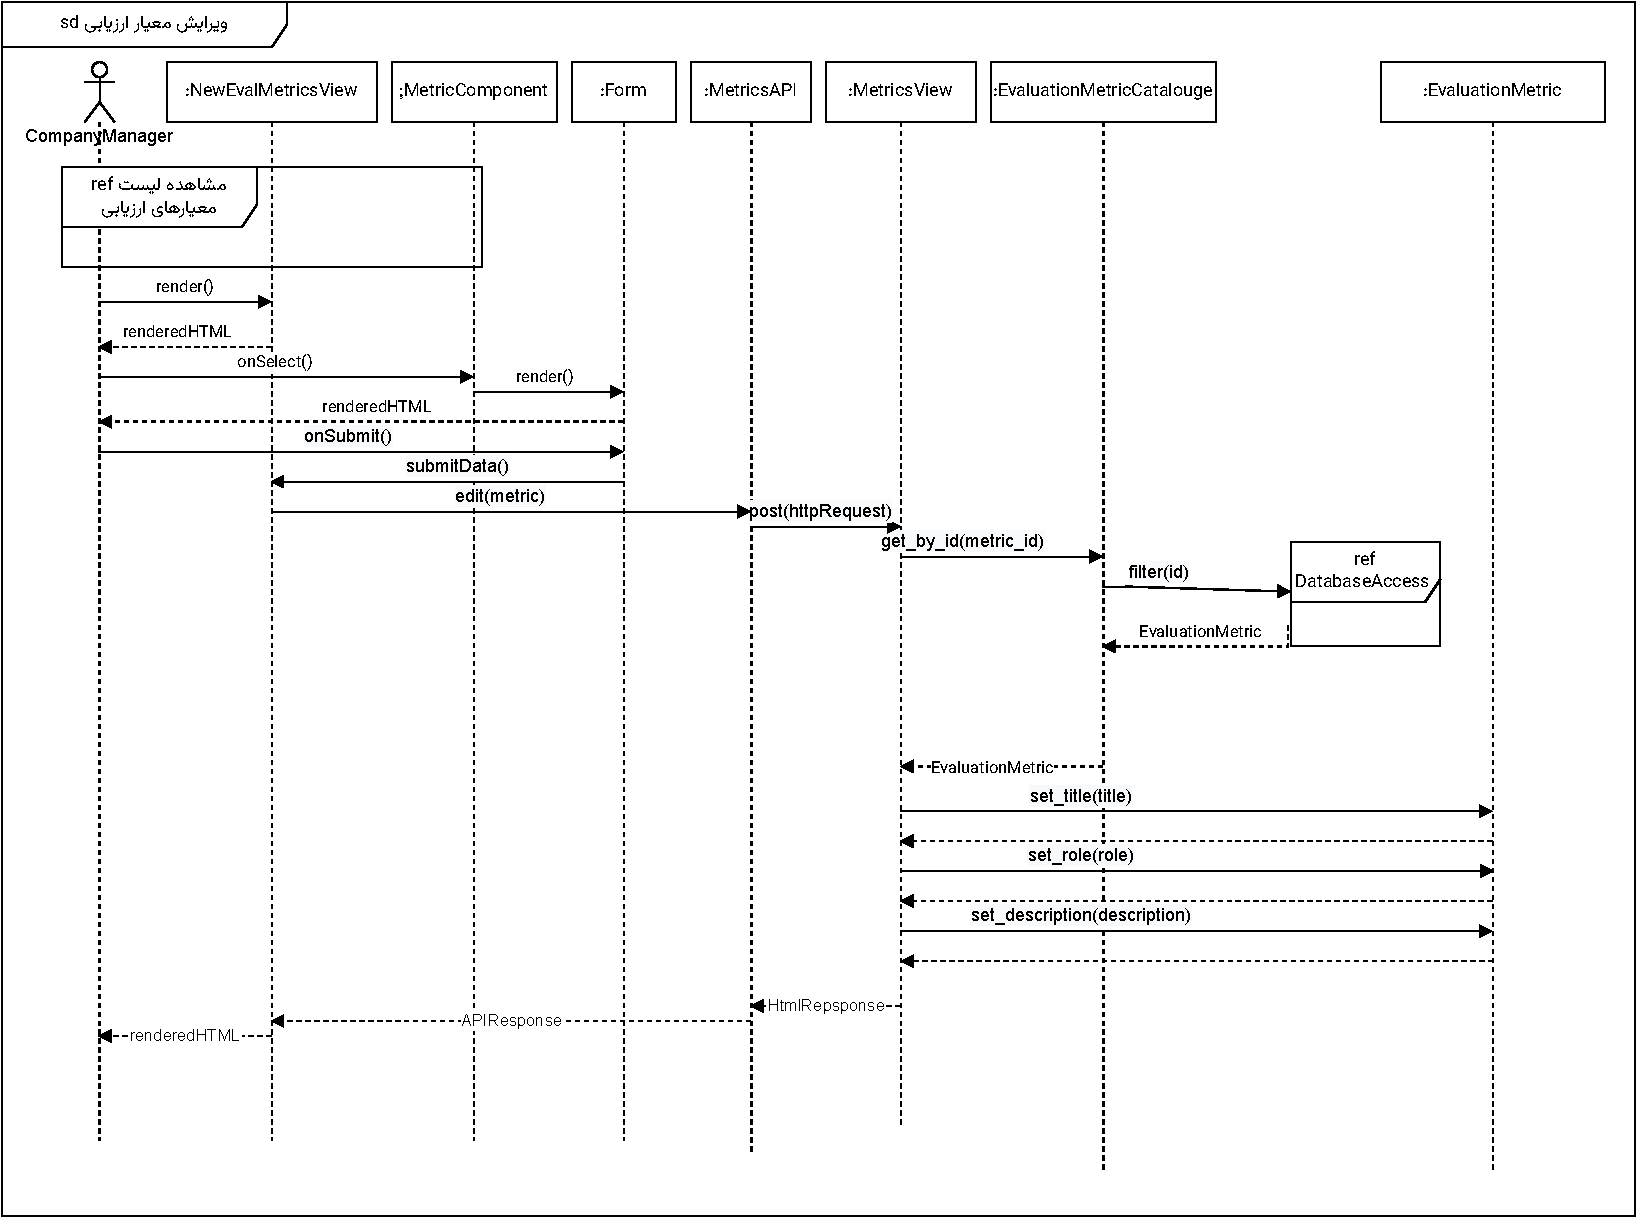
\includegraphics[scale=0.8]{figs/design-sequence/3-28.pdf}
	\caption{نمودار توالی: ویرایش معیار ارزیابی}
\end{figure}
\FloatBarrier
\newpage

\eject \pdfpagewidth=12in \pdfpageheight=11in
\begin{figure}[ht!]
	\centering
	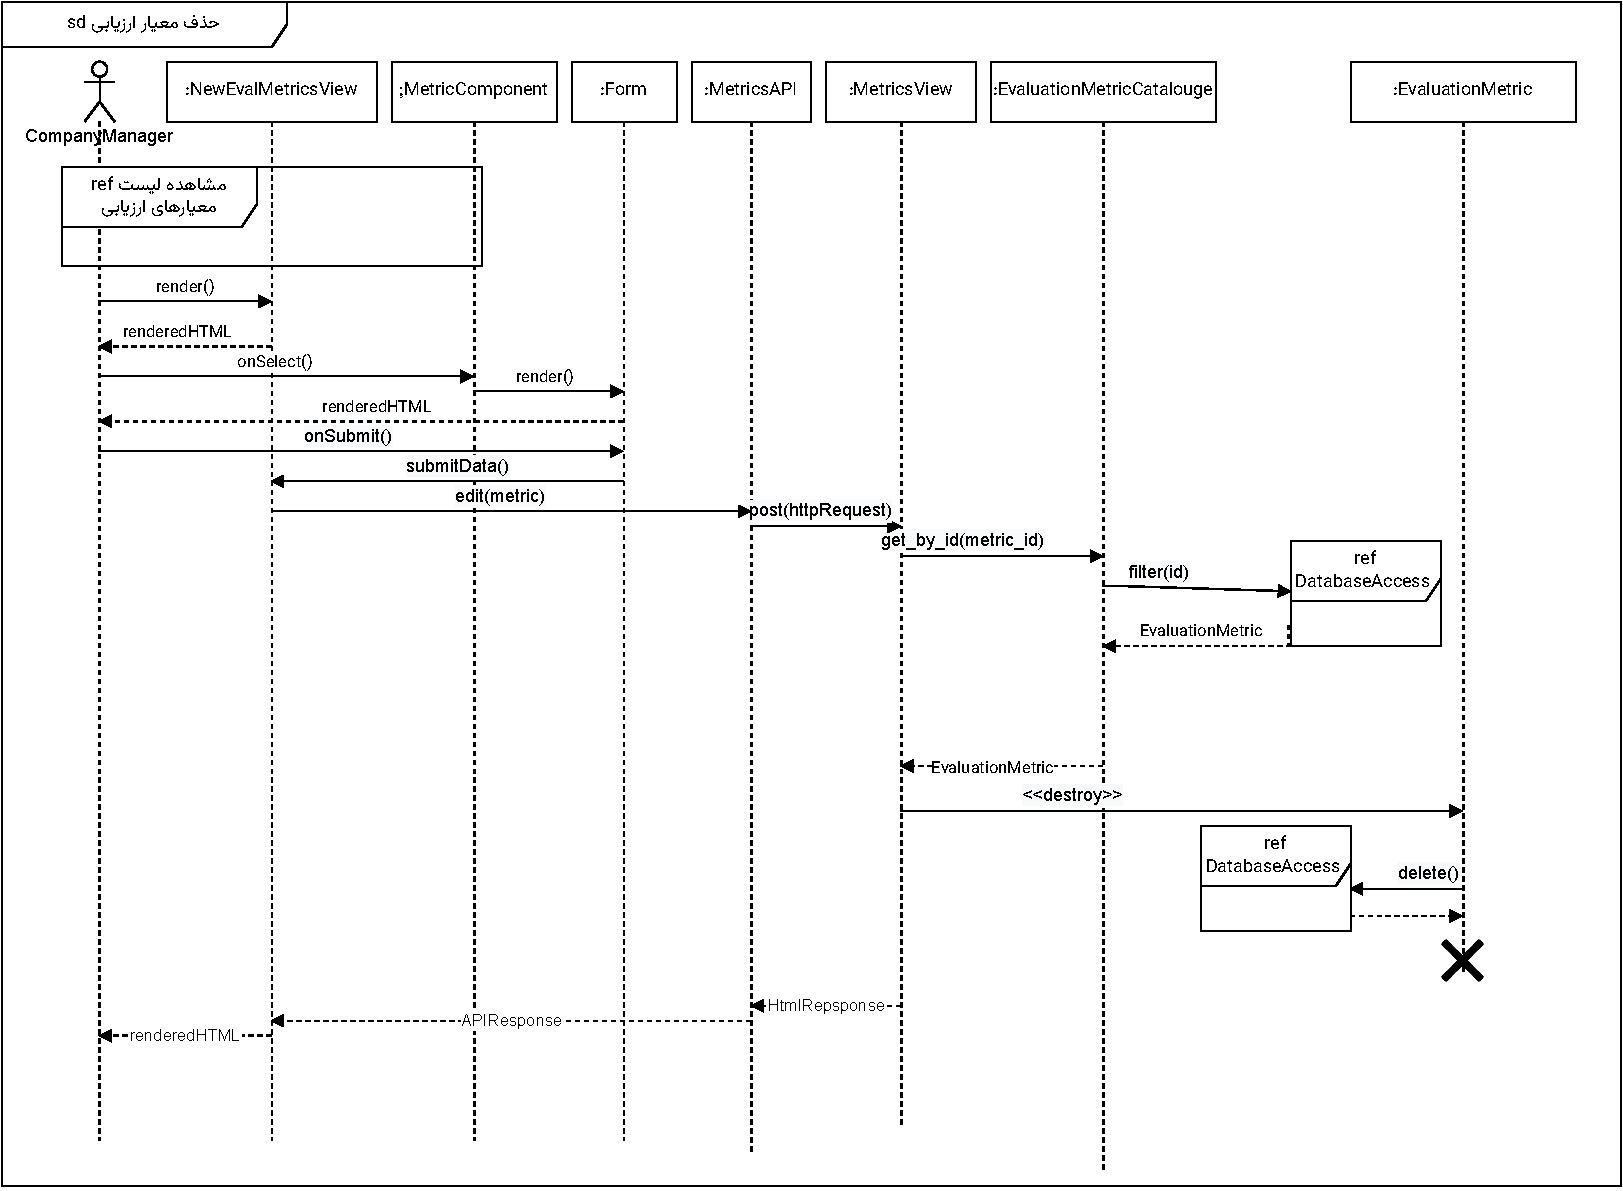
\includegraphics[scale=0.8]{figs/design-sequence/3-29.pdf}
	\caption{نمودار توالی: حذف معیار ارزیابی}
\end{figure}
\FloatBarrier
\newpage

\eject \pdfpagewidth=10in \pdfpageheight=9in

\begin{figure}[ht!]
	\centering
	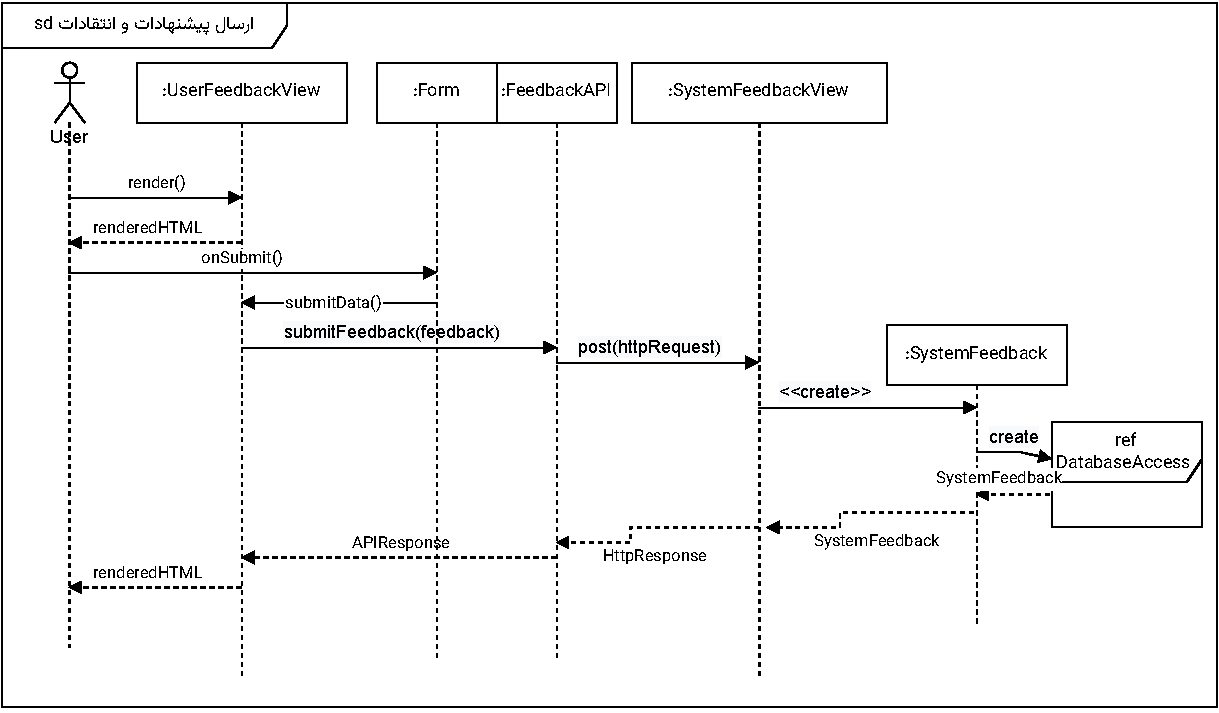
\includegraphics[scale=0.8]{figs/design-sequence/3-30.pdf}
	\caption{نمودار توالی: ارسال پیشنهادات و انتقادات}
\end{figure}

\FloatBarrier
\newpage

\section{زیرسیستم مدیریت}

\eject \pdfpagewidth=15in \pdfpageheight=9in

\FloatBarrier
\begin{figure}[ht!]
	\centering
	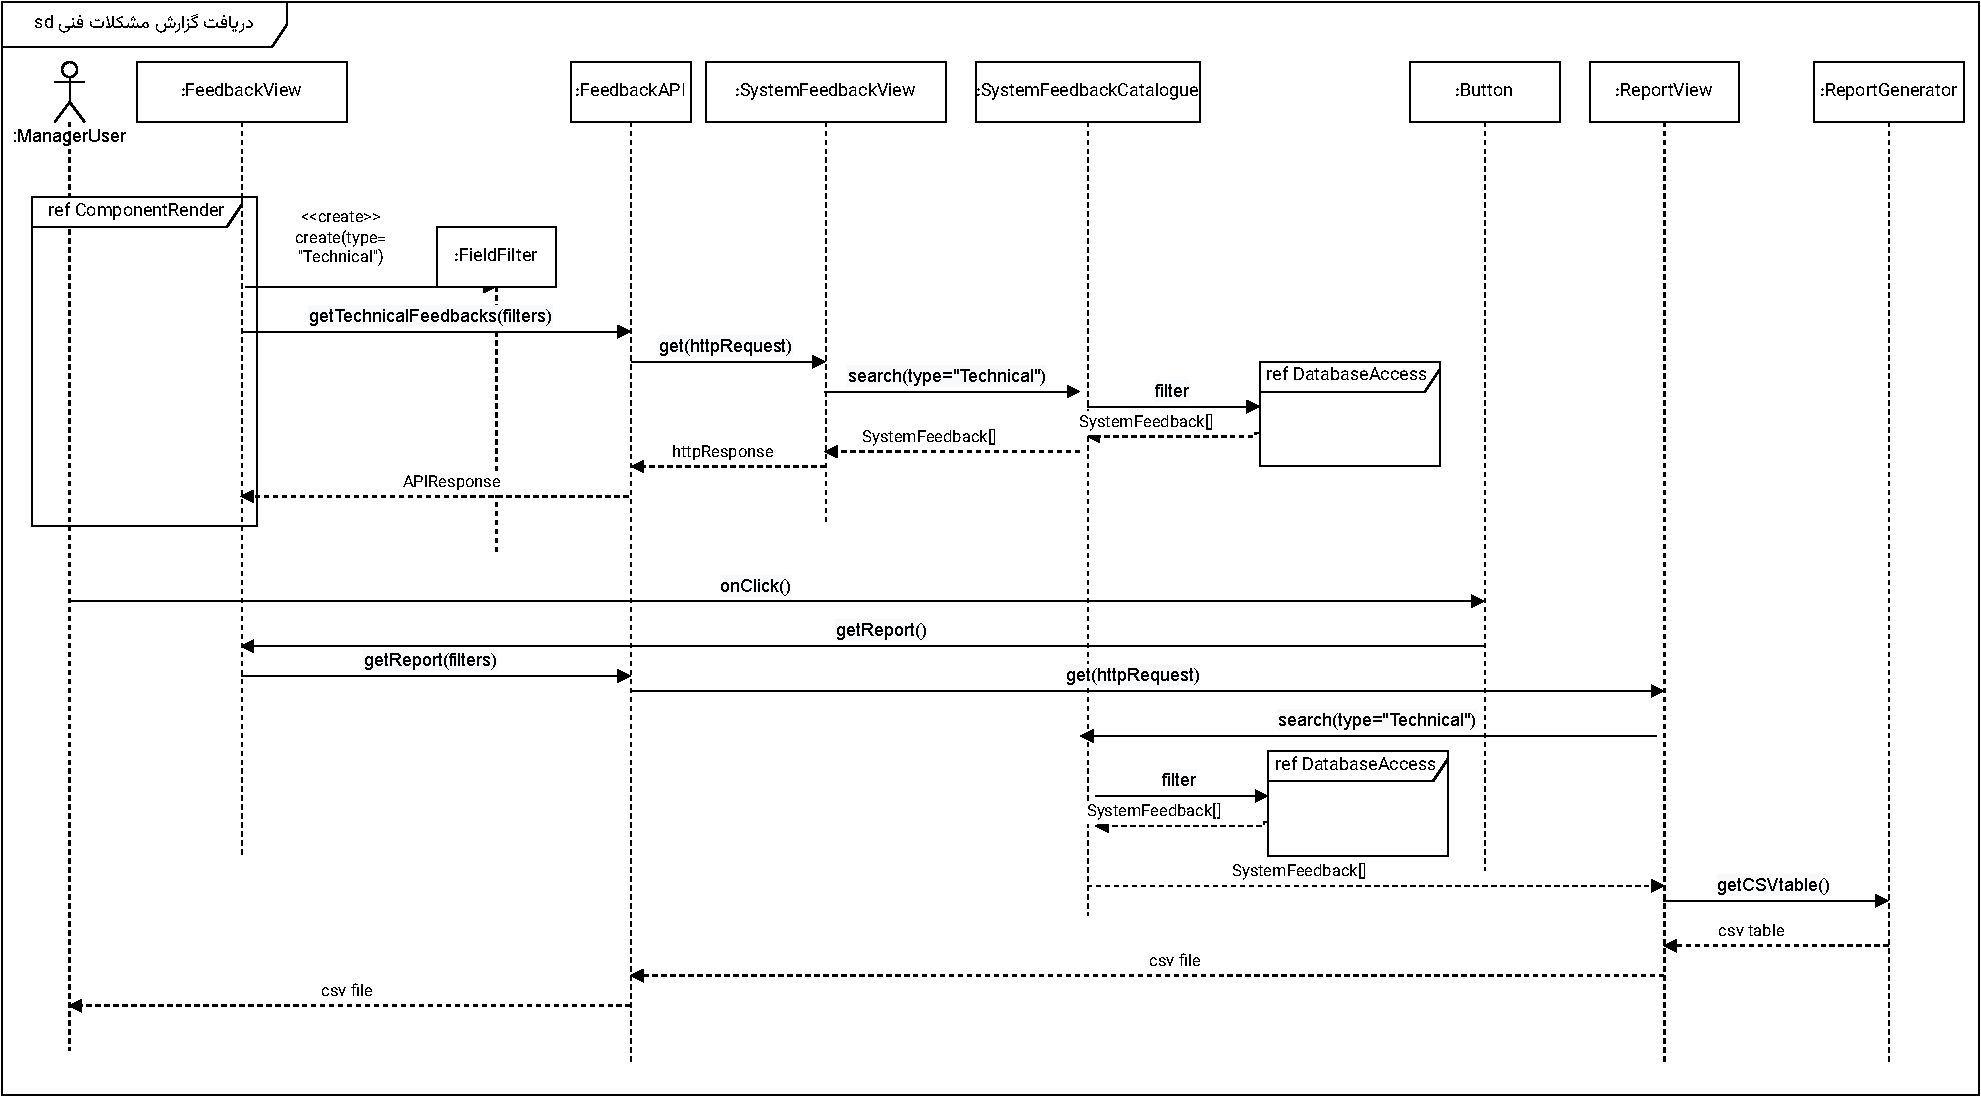
\includegraphics[scale=0.8]{figs/design-sequence/3-39.pdf}
	\caption{نمودار توالی: دریافت گزارش مشکلات فنی}
\end{figure}
\FloatBarrier
\newpage

\eject \pdfpagewidth=12in \pdfpageheight=9in


\begin{figure}[ht!]
	\centering
	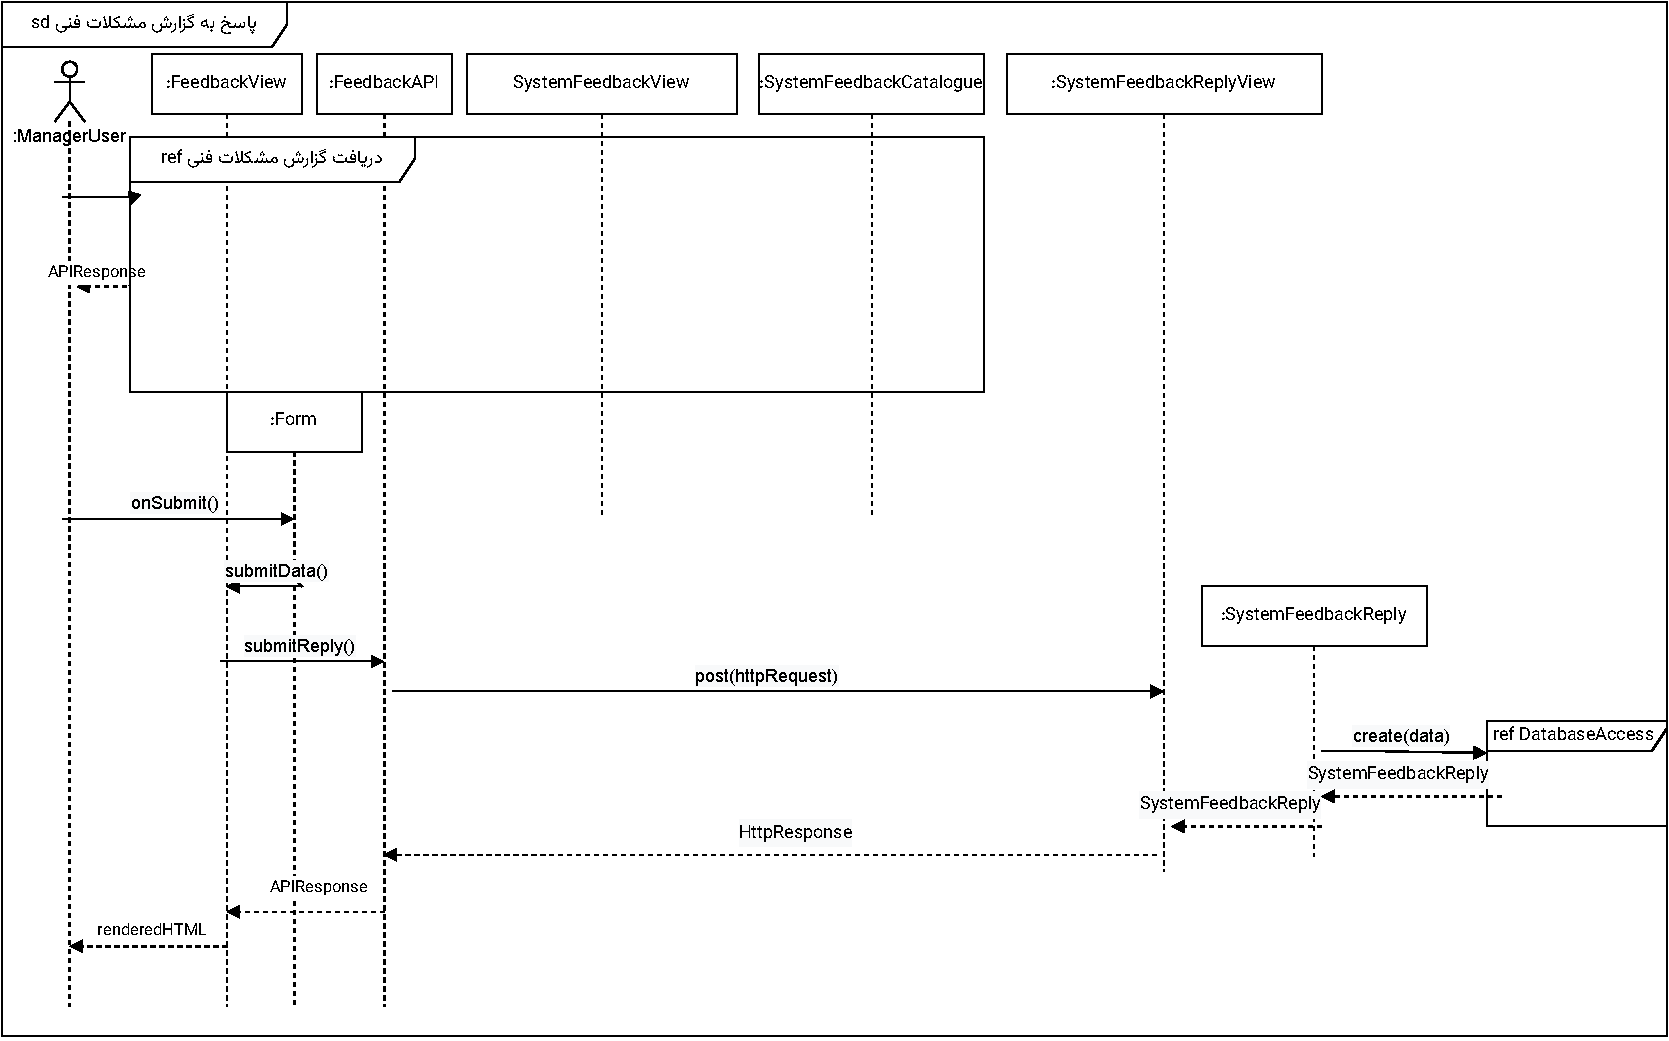
\includegraphics[scale=0.8]{figs/design-sequence/3-40.pdf}
	\caption{نمودار توالی: پاسخ به گزارش مشکلات فنی}
\end{figure}


\KOMAoptions{paper=a4}
\recalctypearea
\newpage
